\documentclass[border=10pt]{standalone}
\usepackage{tikz}
\usepackage{amsmath}
\usetikzlibrary{shapes,arrows,positioning,calc,decorations.pathmorphing,patterns}

\newcommand{\drawDamper}[2]{% #1 = coordinate, #2 = scale factor
  \draw[thick] #1++(0,0) -- ++(0,0.5*#2);
  \draw[thick] #1++(0.5*#2,0) -- ++(0,0.5*#2);
  \draw[thick] #1++(0,0.5*#2) -- ++(0.5*#2,0);
  \draw[thick] #1++(0,0.25*#2) -- ++(0.5*#2,0);
  \draw[thick] #1++(0.25*#2,0.5*#2) -- ++(0,0.5*#2);
  \draw[thick] #1++(0.25*#2,0.25*#2) -- ++(0,-0.5*#2);
}

\newcommand{\floorsize}{3.5}

\begin{document}
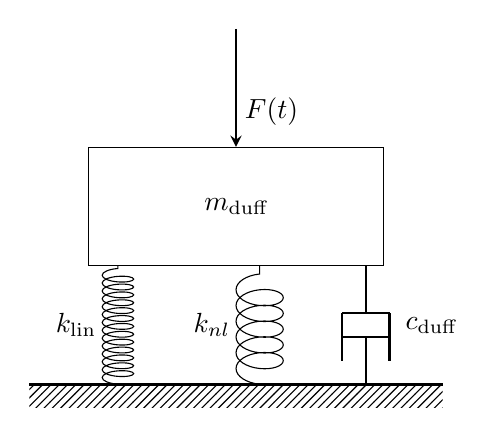
\begin{tikzpicture}[>=stealth, node distance=1cm, scale=1.5]

    % Floor with hatching on top edge only
    \fill[pattern=north east lines, draw=none] (0,0) rectangle ++(\floorsize,-0.2);
    \draw[very thick] (0,0) -- ++(\floorsize,0);

    % Nodes
    % \node (mass) [draw, rectangle, minimum width=2.5cm, minimum height=1cm, anchor=south] at (\floorsize/2,1) {\(m_{\text{duff}}\)};
    \node (mass) [draw, rectangle, minimum width=3.75cm, minimum height=1.5cm, anchor=south] at (\floorsize/2,1) {\(m_{\text{duff}}\)};
    
    % Linear Spring
    \draw[decoration={coil,aspect=0.3, segment length=1mm, amplitude=2mm,coil},decorate] (0.75,0) -- (0.75,1);
    \node[anchor=east, xshift=-0.15cm] at (0.75, 0.5) {\(k_{\text{lin}}\)};
    
    % Nonlinear Spring
    \draw[decoration={coil,aspect=0.5, segment length=2mm, amplitude=3mm,coil},decorate] (1.95,0) -- (1.95,1);
    \node[anchor=east, xshift=-0.25cm] at (1.95, 0.5) {\(k_{nl}\)};
    
    % Damper
    \drawDamper{(2.65, 0.2)}{0.8}
    \node[anchor=west, xshift=0.68cm] at (2.65, 0.5) {\(c_{\text{duff}}\)};
    
    % External Force
    \draw[->, thick] (mass.north) ++ (0,1) -- (mass.north);
    % \node[anchor=south] at (mass.north) {\(F(t)\)};
    % \node[anchor=south] at ($(mass.north) + (0,1)$) {\(F(t)\)};
    % \node[anchor=south] at ($(mass.north) + (0.5,0)$) {\(F(t)\)};
    \node[anchor=south] at ($(mass.north) + (0.30,0.1)$) {\(F(t)\)};

\end{tikzpicture}
\end{document}
